% Created 2022-02-14 Mon 16:17
% Intended LaTeX compiler: pdflatex
\documentclass[presentation,aspectratio=169]{beamer}
\usepackage[utf8]{inputenc}
\usepackage[T1]{fontenc}
\usepackage{graphicx}
\usepackage{grffile}
\usepackage{longtable}
\usepackage{wrapfig}
\usepackage{rotating}
\usepackage[normalem]{ulem}
\usepackage{amsmath}
\usepackage{textcomp}
\usepackage{amssymb}
\usepackage{capt-of}
\usepackage{hyperref}
\usepackage{khpreamble}
\usepackage{amssymb}
\usepgfplotslibrary{groupplots}
\newcommand*{\shift}{\operatorname{q}}
\usetheme{default}
\author{Kjartan Halvorsen}
\date{\today}
\title{Process Automation Laboratory - Modeling first-order systems}
\hypersetup{
 pdfauthor={Kjartan Halvorsen},
 pdftitle={Process Automation Laboratory - Modeling first-order systems},
 pdfkeywords={},
 pdfsubject={},
 pdfcreator={Emacs 26.3 (Org mode 9.4.6)}, 
 pdflang={English}}
\begin{document}

\maketitle

\section{Fitting first-order model}
\label{sec:org3e4b441}
\begin{frame}[label={sec:org5be9d62}]{First-order system example: A tank}
\begin{center}
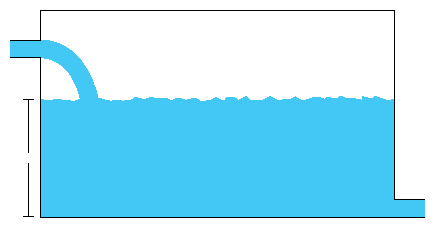
\includegraphics[width=0.7\linewidth]{../../figures/tank-with-hole-no-variables}
\end{center}

\begin{enumerate}
\item What is the \alert{state} of the system?
\item What is the \alert{input signal} and \alert{output signal}?
\end{enumerate}
\end{frame}



\begin{frame}[label={sec:orgf133466}]{First-order system example: A tank}
\begin{center}
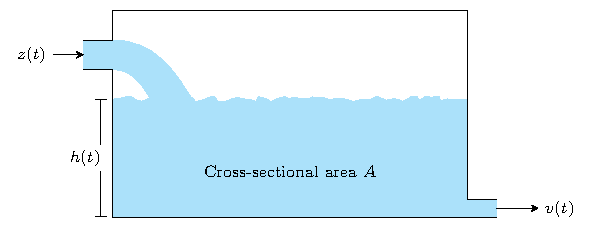
\includegraphics[width=0.7\linewidth]{../../figures/tank-with-hole-simple}
\end{center}

\begin{align*}
\frac{d}{dt} (Ah) &=  z(t) - x(t) = z(t) - a \sqrt{2gh}\quad \Rightarrow\\
\frac{d}{dt} h(t) &= - \frac{a\sqrt{2g}}{A} \sqrt{h(t)} + \frac{1}{A} z(t)
\end{align*}
\end{frame}


\begin{frame}[label={sec:orga98de4f}]{Intuition}
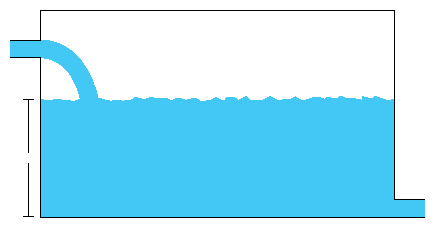
\includegraphics[width=0.2\linewidth]{../../figures/tank-with-hole-no-variables}

\alert{Individual activity} A constant inflow has been present since forever, but at time \(t_1\) the flow in is suddenly shut off. Which of the responses of the water level \(h(t)\) below is correct?

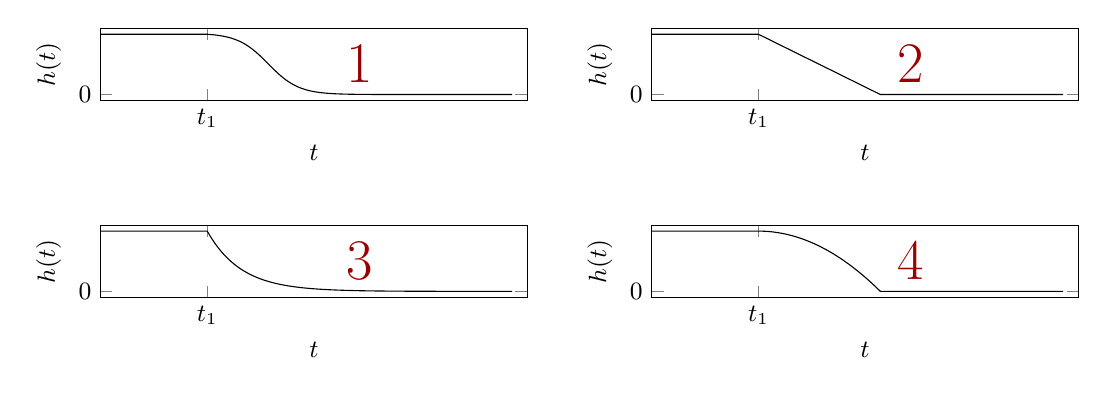
\begin{tikzpicture}
\small

\begin{axis}[
width=7cm,
height=2.5cm,
xlabel={$t$},
ylabel={$h(t)$},
xmin=-3.5,
xmax=10.5,
ytick = {0},
xtick = {0},
xticklabels = {$t_1$},
]
\addplot+[black, no marks, domain=-4:10, samples=400,variable=k] { (k < 0) + (k>0)*(1+exp(-4))/(1+exp(4*(0.5*k-1)))};

\node[black!40!red] at (axis cs: 5, 0.5) {\huge 1};
\end{axis}

\begin{axis}[
xshift=7cm,
width=7cm,
height=2.5cm,
xlabel={$t$},
ylabel={$h(t)$},
xmin=-3.5,
xmax=10.5,
ytick = {0},
xtick = {0},
xticklabels = {$t_1$},
]
\addplot+[black, no marks, domain=-4:10, samples=400,variable=k] { (k<0) + ((k>=0) - (k>4))*(1/4*(4-k)) };
\node[black!40!red] at (axis cs: 5, 0.5) {\huge 2};
\end{axis}

\begin{axis}[
xshift=0cm,
yshift=-2.5cm,
width=7cm,
height=2.5cm,
xlabel={$t$},
ylabel={$h(t)$},
xmin=-3.5,
xmax=10.5,
ytick = {0},
xtick = {0},
xticklabels = {$t_1$},
]
\addplot+[black, no marks, domain=-4:10, samples=400,variable=k] { (k<0) + (k>0)*exp(-0.9*k)};
\node[black!40!red] at (axis cs: 5, 0.5) {\huge 3};
\end{axis}

\begin{axis}[
xshift=7cm,
yshift=-2.5cm,
width=7cm,
height=2.5cm,
xlabel={$t$},
ylabel={$h(t)$},
xmin=-3.5,
xmax=10.5,
ytick = {0},
xtick = {0},
xticklabels = {$t_1$},
]
\addplot+[black, no marks, domain=-4:10, samples=400,variable=k] { (k<0) + ((k>=0) - (k>4))*(1-1/16*pow(-k,2)) };
\node[black!40!red] at (axis cs: 5, 0.5) {\huge 4};
\end{axis}


\end{tikzpicture}
\end{frame}


\begin{frame}[label={sec:org287505b}]{Deviation variables}
\begin{center}
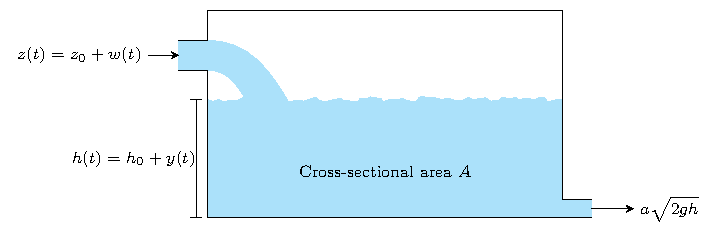
\includegraphics[width=0.7\linewidth]{../../figures/tank-with-hole}
\end{center}

Flow in: \(z(t) = z_0 + w(t)\). Level of water: \(h(t) = h_0 + y(t)\). The constants \(h_0\) and \(z_0\) define an \emph{operating point}.

\begin{align*}
\frac{d}{dt} h(t) &= - \frac{a\sqrt{2g}}{A} \sqrt{h(t)} + \frac{1}{A} z(t)
\end{align*}


\alert{Individual activity} Given \(h_0\) determine the operating point for the inflow, \(z_0\), such that the system is in equilibrium at the operating point.
\end{frame}

\begin{frame}[label={sec:orga0fe692}]{Intuition}
Which change \(y(t)\) in the water level corresponds to a step change \(w(t)\) in the inflow? 

\begin{center}
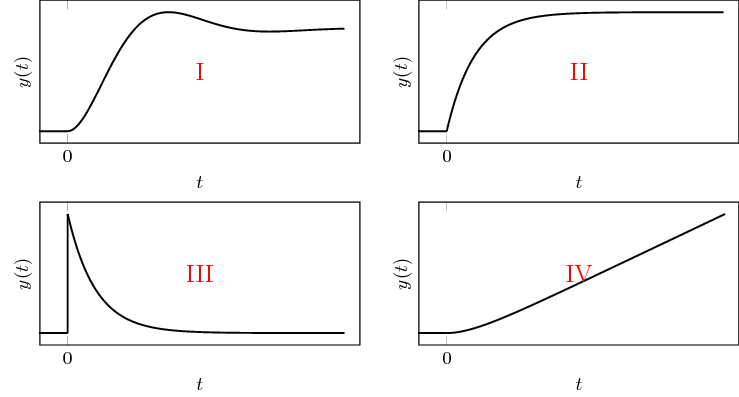
\includegraphics[width=0.7\linewidth]{../../figures/dc-response-exercise}
\end{center}
\end{frame}



\begin{frame}[label={sec:org18de56c}]{Fitting a first-order model}
Assuming a plant model of first-order with time-constant \(T\)
\[  \quad \textcolor{green!50!black}{Y(s)} = \frac{K}{sT + 1}\textcolor{blue!80!black}{U(s)} \quad \overset{U(s) = \frac{u_f}{s}}{\Longrightarrow} \quad \textcolor{green!50!black}{y(t)} = u_f K\big( 1 - \mathrm{e}^{-\frac{t}{T}}\big)u_H(t)\]
\def\Tcnst{3}
\def\tdelay{0.0}
\def\ggain{2}
\def\uampl{0.8}
\pgfmathsetmacro{\yfinal}{\uampl*\ggain}
\pgfmathsetmacro{\yone}{0.283*\yfinal}
\pgfmathsetmacro{\ytwo}{0.632*\yfinal}
\pgfmathsetmacro{\tone}{\tdelay + \Tcnst/3}
\pgfmathsetmacro{\two}{\tdelay + \Tcnst}

\begin{center}
  \begin{tikzpicture}
    \begin{axis}[
    width=14cm,
    height=4.5cm,
    grid = both,
    xtick = {0,  \two},
    xticklabels = {0, $T$},
    ytick = {0, \ytwo, \uampl, \yfinal},
    yticklabels = {0,  $ $, $u_f$, $y_f$},
    xmin = -0.2,
    %minor y tick num=9,
    %minor x tick num=9,
    %every major grid/.style={red, opacity=0.5},
    xlabel = {$t$},
    ]
      \addplot [thick, green!50!black, no marks, domain=0:10, samples=100] {\uampl*\ggain*(x>\tdelay)*(1 - exp(-(x-\tdelay)/\Tcnst)} node [coordinate, pos=0.9, pin=-90:{$y(t)$}] {};
      \addplot [const plot, thick, blue!80!black, no marks, domain=-1:10, samples=100] coordinates {(-1,0) (0,0) (0,\uampl) (10,\uampl)} node [coordinate, pos=0.9, pin=-90:{$u(t)$}] {};
    \end{axis}
  \end{tikzpicture}
\end{center}

\alert{Individual activity} Evaluate the response \(y(t)\) at the time instant \(t=T\) and for \(t\to\infty\)!
\end{frame}

\begin{frame}[label={sec:org90be63e}]{Fitting a first-order model}
Assuming a plant model of first-order with time-constant \(T\)
\[  \quad \textcolor{green!50!black}{Y(s)} = \frac{K}{sT + 1}\textcolor{blue!80!black}{U(s)} \quad \overset{U(s) = \frac{u_f}{s}}{\Longrightarrow} \quad \textcolor{green!50!black}{y(t)} = u_f K\big( 1 - \mathrm{e}^{-\frac{t}{T}}\big)u_H(t)\]
\def\Tcnst{3}
\def\tdelay{0.0}
\def\ggain{2}
\def\uampl{0.8}
\pgfmathsetmacro{\yfinal}{\uampl*\ggain}
\pgfmathsetmacro{\yone}{0.283*\yfinal}
\pgfmathsetmacro{\ytwo}{0.632*\yfinal}
\pgfmathsetmacro{\tone}{\tdelay + \Tcnst/3}
\pgfmathsetmacro{\two}{\tdelay + \Tcnst}

\begin{center}
  \small
  \begin{tikzpicture}
    \begin{axis}[
    width=14cm,
    height=3.5cm,
    grid = both,
    xtick = {0,  \two},
    xticklabels = {0, $T$},
    ytick = {0, \ytwo, \uampl, \yfinal},
    yticklabels = {0,  $0.632y_f$, $u_f$, $y_f$},
    xmin = -0.2,
    %minor y tick num=9,
    %minor x tick num=9,
    %every major grid/.style={red, opacity=0.5},
    xlabel = {$t$},
    ]
      \addplot [thick, green!50!black, no marks, domain=0:10, samples=100] {\uampl*\ggain*(x>\tdelay)*(1 - exp(-(x-\tdelay)/\Tcnst)} node [coordinate, pos=0.9, pin=-90:{$y(t)$}] {};
      \addplot [const plot, thick, blue!80!black, no marks, domain=-1:10, samples=100] coordinates {(-1,0) (0,0) (0,\uampl) (10,\uampl)} node [coordinate, pos=0.9, pin=-90:{$u(t)$}] {};
    \end{axis}
  \end{tikzpicture}
\end{center}

\alert{Time-constant:} Find the time \(t=T\) at which the response has reached 63.2\% of its final value

\alert{Gain:} \(y_f = \lim_{t\to\infty}y(t) = Ku_f \quad \Rightarrow \quad K = \frac{y_f}{u_f}\)
\end{frame}


\section{CSTR}
\label{sec:orgf15baf4}

\begin{frame}[label={sec:org8673876}]{A Continuous Stirred Tank Reactor}
\begin{center}
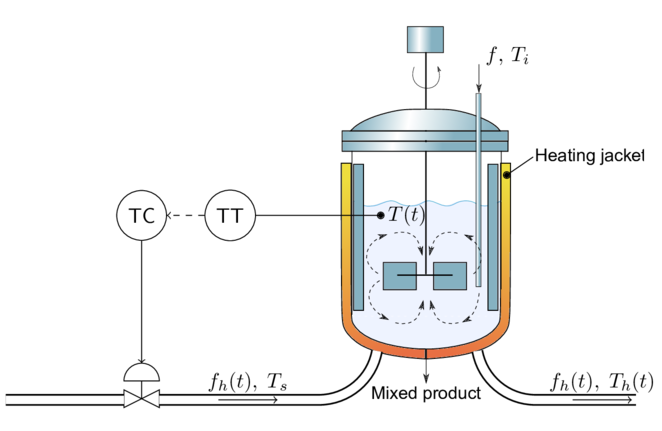
\includegraphics[height=0.8\textheight]{../../figures/stirred_tank_heat_exchange}
\end{center}
\end{frame}

\begin{frame}[label={sec:org1afa60f}]{A Continuous Stirred Tank Reactor}
\begin{columns}
\begin{column}{0.6\columnwidth}
\begin{center}
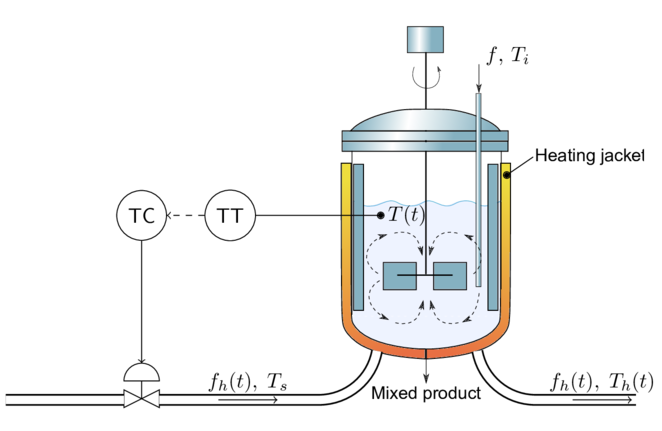
\includegraphics[height=0.6\textheight]{../../figures/stirred_tank_heat_exchange}
\end{center}
\end{column}

\begin{column}{0.4\columnwidth}
Assume:
\begin{enumerate}
\item Constant flow \(f\) through the tank reactor
\item Constant temperatures \(T_i\) and \(T_s\)
\item Perfect mixing in the tank reactor
\item Perfect mixing in the heating jacket
\item Isothermic reaction
\end{enumerate}
\end{column}
\end{columns}
\end{frame}

\begin{frame}[label={sec:org5610c92}]{A Continuous Stirred Tank Reactor}
\begin{center}
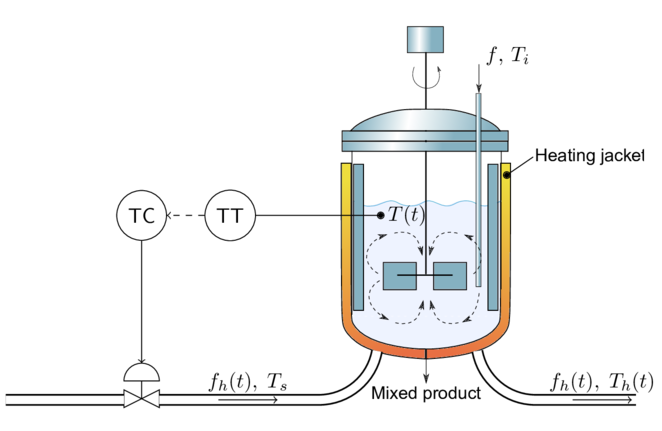
\includegraphics[height=0.4\textheight]{../../figures/stirred_tank_heat_exchange}
\end{center}

Energy balance:
\begin{align*}
\frac{dT(t)}{dt} &= k_1\big( T_i - T(t) \big) + k_2 \big( T_h(t) - T(t)\big)\\
\frac{dT_h(t)}{dt} &= k_3f_h(t)\big( T_s - T_h(t) \big) - k_4 \big( T_h(t) - T(t)\big)
\end{align*}
\end{frame}



\begin{frame}[label={sec:orgb7fa36e}]{Intuition}
\begin{center}
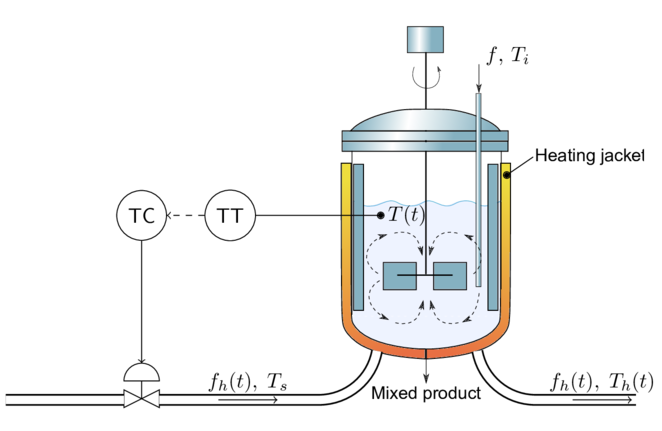
\includegraphics[height=0.3\textheight]{../../figures/stirred_tank_heat_exchange}
\end{center}

\begin{center}
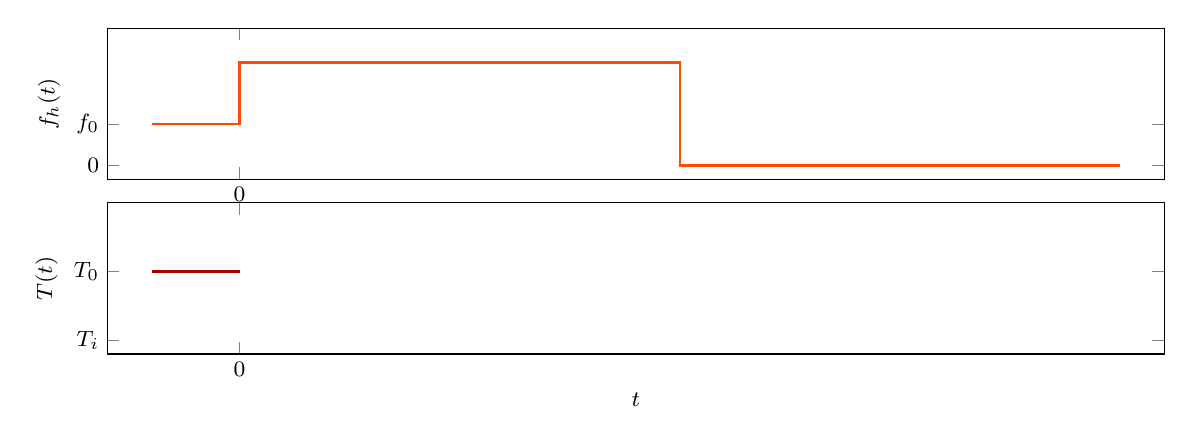
\begin{tikzpicture}
    \footnotesize

    \pgfmathsetmacro{\fnull}{0.6}
    \pgfmathsetmacro{\fstep}{1.5}
    \pgfmathsetmacro{\Tnull}{1}
    \pgfmathsetmacro{\Ti}{0}

    \begin{groupplot}[group style={group size=1 by 2, vertical sep=0.3cm, horizontal sep=1.3cm},
    width=15cm,
    height=3.5cm,
    xlabel={$t$},
    xmin=-1.5,
    xmax=10.5,
    ytick = \empty,
    xtick = {0},
    ymin=-0.2, ymax=2,
    ]
    \nextgroupplot[ytick={ 0, \fnull}, 
    yticklabels={0, $f_0$,}, ylabel={$f_h(t)$}, xlabel={},]
    \addplot[orange!60!red, thick,] coordinates { (-1, \fnull) (0,\fnull) (0,\fstep) (5,\fstep) (5,0) (10,0)};
    \nextgroupplot[ytick={ \Ti, \Tnull}, 
    yticklabels={$T_i$, $T_0$,}, ylabel={$T(t)$}]
    \addplot[red!60!black, thick, ] coordinates { (-1, \Tnull) (0,\Tnull)};

    \end{groupplot}
  \end{tikzpicture}
\end{center}
\end{frame}


\section{Fitting first-order model with delay}
\label{sec:org7256e37}
\begin{frame}[label={sec:org25e96b5}]{Fitting first-order model with delay}
Assuming a plant model of first-order with time constant \(T\) and delay \(\tau\)
\[  \quad \textcolor{green!50!black}{Y(s)} = \frac{K\mathrm{e}^{-s\tau}}{sT + 1}\textcolor{blue!80!black}{U(s)} \quad \overset{U(s) = \frac{u_f}{s}}{\Longrightarrow} \quad \textcolor{green!50!black}{y(t)} = u_f K\big( 1 - \mathrm{e}^{-\frac{t-\tau}{T}}\big)u_H(t-\tau)\]
\def\Tcnst{3}
\def\tdelay{0.6}
\def\ggain{2}
\def\uampl{0.8}
\pgfmathsetmacro{\yfinal}{\uampl*\ggain}
\pgfmathsetmacro{\yone}{0.283*\yfinal}
\pgfmathsetmacro{\ytwo}{0.632*\yfinal}
\pgfmathsetmacro{\tone}{\tdelay + \Tcnst/3}
\pgfmathsetmacro{\two}{\tdelay + \Tcnst}

\begin{center}
  \begin{tikzpicture}
    \begin{axis}[
    width=14cm,
    height=4.5cm,
    grid = both,
    xtick = {0, \tdelay, \tone, \two},
    xticklabels = {0, $\tau$, $\tau+\frac{T}{3}$, $\tau + T$},
    ytick = {0, \yone, \ytwo, \uampl, \yfinal},
    yticklabels = {0, $ $, $ $, $u_f$, $y_f$},
    xmin = -0.2,
    %minor y tick num=9,
    %minor x tick num=9,
    %every major grid/.style={red, opacity=0.5},
    xlabel = {$t$},
    ]
      \addplot [thick, green!50!black, no marks, domain=0:10, samples=100] {\uampl*\ggain*(x>\tdelay)*(1 - exp(-(x-\tdelay)/\Tcnst)} node [coordinate, pos=0.9, pin=-90:{$y(t)$}] {};
      \addplot [const plot, thick, blue!80!black, no marks, domain=-1:10, samples=100] coordinates {(-1,0) (0,0) (0,\uampl) (10,\uampl)} node [coordinate, pos=0.9, pin=-90:{$u(t)$}] {};
    \end{axis}
  \end{tikzpicture}
\end{center}

\alert{Individual activity} Evaluate the response \(y(t)\) at the two time instants \(t=\tau + \frac{T}{3}\) and \(t=\tau + T\)!
\end{frame}


\begin{frame}[label={sec:org549b156}]{Fitting first-order model with delay}
Assuming a plant model of first-order with time constant \(T\) and delay \(\tau\)
\[  \quad \textcolor{green!50!black}{Y(s)} = \frac{K\mathrm{e}^{-s\tau}}{sT + 1}\textcolor{blue!80!black}{U(s)} \quad \overset{U(s) = \frac{u_f}{s}}{\Longrightarrow} \quad \textcolor{green!50!black}{y(t)} = u_f K\big( 1 - \mathrm{e}^{-\frac{t-\tau}{T}}\big)u_H(t-\tau)\]
\def\Tcnst{3}
\def\tdelay{0.6}
\def\ggain{2}
\def\uampl{0.8}
\pgfmathsetmacro{\yfinal}{\uampl*\ggain}
\pgfmathsetmacro{\yone}{0.283*\yfinal}
\pgfmathsetmacro{\ytwo}{0.632*\yfinal}
\pgfmathsetmacro{\tone}{\tdelay + \Tcnst/3}
\pgfmathsetmacro{\two}{\tdelay + \Tcnst}

\begin{center}
  \begin{tikzpicture}
    \begin{axis}[
    width=14cm,
    height=4.5cm,
    grid = both,
    xtick = {0, \tdelay, \tone, \two},
    xticklabels = {0, $\tau$, $\tau+\frac{T}{3}$, $\tau + T$},
    ytick = {0, \yone, \ytwo, \uampl, \yfinal},
    yticklabels = {0, $0.283y_{f}$, $0.632y_f$, $u_f$, $y_f$},
    xmin = -0.2,
    %minor y tick num=9,
    %minor x tick num=9,
    %every major grid/.style={red, opacity=0.5},
    xlabel = {$t$},
    ]
      \addplot [thick, green!50!black, no marks, domain=0:10, samples=100] {\uampl*\ggain*(x>\tdelay)*(1 - exp(-(x-\tdelay)/\Tcnst)} node [coordinate, pos=0.9, pin=-90:{$y(t)$}] {};
      \addplot [const plot, thick, blue!80!black, no marks, domain=-1:10, samples=100] coordinates {(-1,0) (0,0) (0,\uampl) (10,\uampl)} node [coordinate, pos=0.9, pin=-90:{$u(t)$}] {};
    \end{axis}
  \end{tikzpicture}
\end{center}

\[ y_f = \lim_{t\to\infty} y(t) = u_f K \quad \Rightarrow \quad K = \frac{y_f}{u_f}. \]
\end{frame}

\begin{frame}[label={sec:orgfac1186}]{First-order model with delay - example}
\[  \quad Y(s) = \frac{K\mathrm{e}^{-s\tau}}{sT + 1}U(s) \quad \overset{U(s) = \frac{u_f}{s}}{\Longrightarrow} \quad y(t) = u_f K\big( 1 - \mathrm{e}^{-\frac{t-\tau}{T}}\big)u_s(t-\tau)\]
\def\Tcnst{2.1}
\def\tdelay{1}
\def\ggain{2}
\def\uampl{0.8}
\pgfmathsetmacro{\yfinal}{\uampl*\ggain}
\pgfmathsetmacro{\yone}{0.283*\yfinal}
\pgfmathsetmacro{\ytwo}{0.632*\yfinal}
\pgfmathsetmacro{\tone}{\tdelay + \Tcnst/3}
\pgfmathsetmacro{\two}{\tdelay + \Tcnst}

\begin{center}
  \begin{tikzpicture}
    \begin{axis}[
    width=12cm,
    height=4cm,
    grid = both,
    %xtick = {0, \tdelay, \tone, \two},
    %xticklabels = {0, $\tau$, $\tau+\frac{T}{3}$, $\tau + T$},
    %ytick = {0, \yone, \ytwo, \uampl, \yfinal},
    %yticklabels = {0, $0.283y_{f}$, $0.632y_f$, $u_f$, $y_f$},
    xmin = -0.2,
    minor y tick num=9,
    minor x tick num=9,
    every major grid/.style={red, opacity=0.5},
    %xlabel = {$t$},
    clip = false,
    ]
      \addplot [thick, green!50!black, smooth, no marks, domain=0:10, samples=16] {\uampl*\ggain*(x>\tdelay)*(1 - exp(-(x-\tdelay)/\Tcnst)} node [coordinate, pos=0.9, pin=-90:{$y(t)$}] {};
      \addplot [const plot, thick, blue!80!black, no marks, domain=-1:10, samples=100] coordinates {(-1,0) (0,0) (0,\uampl) (10,\uampl)} node [coordinate, pos=0.9, pin=-90:{$u(t)$}] {};
      \draw[thick, green!70!black, dashed] (axis cs: 10, \yfinal) -- (axis cs: -1, \yfinal, -0.9) node[left, anchor=east] {$y_f = \yfinal$}; 
      \draw[blue!70!black, dashed] (axis cs: 0, \uampl) -- (axis cs: -1, \uampl, -0.9) node[left, anchor=east] {$u_f = \uampl$}; 
    \end{axis}
  \end{tikzpicture}
\end{center}
\end{frame}

\begin{frame}[label={sec:org94303f6}]{First-order model with delay - example}
\[  \quad Y(s) = \frac{K\mathrm{e}^{-s\tau}}{sT + 1}U(s) \quad \overset{U(s) = \frac{u_f}{s}}{\Longrightarrow} \quad y(t) = u_f K\big( 1 - \mathrm{e}^{-\frac{t-\tau}{T}}\big)u_s(t-\tau)\]
\def\Tcnst{2.1}
\def\tdelay{1}
\def\ggain{2}
\def\uampl{0.8}
\pgfmathsetmacro{\yfinal}{\uampl*\ggain}
\pgfmathsetmacro{\yone}{0.283*\yfinal}
\pgfmathsetmacro{\ytwo}{0.632*\yfinal}
\pgfmathsetmacro{\tone}{\tdelay + \Tcnst/3}
\pgfmathsetmacro{\two}{\tdelay + \Tcnst}

\begin{center}
  \begin{tikzpicture}
    \begin{axis}[
    width=12cm,
    height=4cm,
    grid = both,
    %xtick = {0, \tdelay, \tone, \two},
    %xticklabels = {0, $\tau$, $\tau+\frac{T}{3}$, $\tau + T$},
    %ytick = {0, \yone, \ytwo, \uampl, \yfinal},
    %yticklabels = {0, $0.283y_{f}$, $0.632y_f$, $u_f$, $y_f$},
    xmin = -0.2,
    minor y tick num=9,
    minor x tick num=9,
    every major grid/.style={red, opacity=0.5},
    %xlabel = {$t$},
    clip = false,
    ]
      \addplot [thick, green!50!black, smooth, no marks, domain=0:10, samples=16] {\uampl*\ggain*(x>\tdelay)*(1 - exp(-(x-\tdelay)/\Tcnst)} node [coordinate, pos=0.9, pin=-90:{$y(t)$}] {};
      \addplot [const plot, thick, blue!80!black, no marks, domain=-1:10, samples=100] coordinates {(-1,0) (0,0) (0,\uampl) (10,\uampl)} node [coordinate, pos=0.9, pin=-90:{$u(t)$}] {};
      \draw[thick, orange, dashed] (axis cs: \two, \ytwo) -- (axis cs: \two, -0.9) node[below] {$t_2 = \two = \tau + T$}; 
      \draw[thick, orange, dashed] (axis cs: \two, \ytwo) -- (axis cs: -1, \ytwo, -0.9) node[left, anchor=east] {$0.632y_f = \ytwo$}; 
      \draw[thick, green!70!black, dashed] (axis cs: 10, \yfinal) -- (axis cs: -1, \yfinal, -0.9) node[left, anchor=east] {$y_f = \yfinal$}; 
      \draw[blue!70!black, dashed] (axis cs: 0, \uampl) -- (axis cs: -1, \uampl, -0.9) node[left, anchor=east] {$u_f = \uampl$}; 
    \end{axis}
  \end{tikzpicture}
\end{center}
\end{frame}

\begin{frame}[label={sec:org6f7bdb2}]{First-order model with delay - example}
\[  \quad Y(s) = \frac{K\mathrm{e}^{-s\tau}}{sT + 1}U(s) \quad \overset{U(s) = \frac{u_f}{s}}{\Longrightarrow} \quad y(t) = u_f K\big( 1 - \mathrm{e}^{-\frac{t-\tau}{T}}\big)u_s(t-\tau)\]
\def\Tcnst{2.1}
\def\tdelay{1}
\def\ggain{2}
\def\uampl{0.8}
\pgfmathsetmacro{\yfinal}{\uampl*\ggain}
\pgfmathsetmacro{\yone}{0.283*\yfinal}
\pgfmathsetmacro{\ytwo}{0.632*\yfinal}
\pgfmathsetmacro{\tone}{\tdelay + \Tcnst/3}
\pgfmathsetmacro{\two}{\tdelay + \Tcnst}

\begin{center}
  \begin{tikzpicture}
    \begin{axis}[
    width=12cm,
    height=4cm,
    grid = both,
    %xtick = {0, \tdelay, \tone, \two},
    %xticklabels = {0, $\tau$, $\tau+\frac{T}{3}$, $\tau + T$},
    %ytick = {0, \yone, \ytwo, \uampl, \yfinal},
    %yticklabels = {0, $0.283y_{f}$, $0.632y_f$, $u_f$, $y_f$},
    xmin = -0.2,
    minor y tick num=9,
    minor x tick num=9,
    every major grid/.style={red, opacity=0.5},
    %xlabel = {$t$},
    clip = false,
    ]
      \addplot [thick, green!50!black, smooth, no marks, domain=0:10, samples=16] {\uampl*\ggain*(x>\tdelay)*(1 - exp(-(x-\tdelay)/\Tcnst)} node [coordinate, pos=0.9, pin=-90:{$y(t)$}] {};
      \addplot [const plot, thick, blue!80!black, no marks, domain=-1:10, samples=100] coordinates {(-1,0) (0,0) (0,\uampl) (10,\uampl)} node [coordinate, pos=0.9, pin=-90:{$u(t)$}] {};
      \draw[thick, red, dashed] (axis cs: \tone, \yone) -- (axis cs: \tone, -0.45) node[below] {$t_1 = \tone = \tau + \frac{T}{3}$}; 
      \draw[thick, red, dashed] (axis cs: \tone, \yone) -- (axis cs: -1,\yone) node[left, anchor=east] {$0.283y_f = \yone$}; 
      \draw[thick, orange, dashed] (axis cs: \two, \ytwo) -- (axis cs: \two, -0.9) node[below] {$t_2 = \two = \tau + T$}; 
      \draw[thick, orange, dashed] (axis cs: \two, \ytwo) -- (axis cs: -1, \ytwo, -0.9) node[left, anchor=east] {$0.632y_f = \ytwo$}; 
      \draw[thick, green!70!black, dashed] (axis cs: 10, \yfinal) -- (axis cs: -1, \yfinal, -0.9) node[left, anchor=east] {$y_f = \yfinal$}; 
      \draw[blue!70!black, dashed] (axis cs: 0, \uampl) -- (axis cs: -1, \uampl, -0.9) node[left, anchor=east] {$u_f = \uampl$}; 
    \end{axis}
  \end{tikzpicture}
\end{center}
\end{frame}

\begin{frame}[label={sec:org30baf93}]{First-order model with delay - example}
\[  \quad Y(s) = \frac{K\mathrm{e}^{-s\tau}}{sT + 1}U(s) \quad \overset{U(s) = \frac{u_f}{s}}{\Longrightarrow} \quad y(t) = u_f K\big( 1 - \mathrm{e}^{-\frac{t-\tau}{T}}\big)u_s(t-\tau)\]
\def\Tcnst{2.1}
\def\tdelay{1}
\def\ggain{2}
\def\uampl{0.8}
\pgfmathsetmacro{\yfinal}{\uampl*\ggain}
\pgfmathsetmacro{\yone}{0.283*\yfinal}
\pgfmathsetmacro{\ytwo}{0.632*\yfinal}
\pgfmathsetmacro{\tone}{\tdelay + \Tcnst/3}
\pgfmathsetmacro{\two}{\tdelay + \Tcnst}

\begin{center}
  \begin{tikzpicture}
    \begin{axis}[
    width=12cm,
    height=4cm,
    grid = both,
    %xtick = {0, \tdelay, \tone, \two},
    %xticklabels = {0, $\tau$, $\tau+\frac{T}{3}$, $\tau + T$},
    %ytick = {0, \yone, \ytwo, \uampl, \yfinal},
    %yticklabels = {0, $0.283y_{f}$, $0.632y_f$, $u_f$, $y_f$},
    xmin = -0.2,
    minor y tick num=9,
    minor x tick num=9,
    every major grid/.style={red, opacity=0.5},
    %xlabel = {$t$},
    clip = false,
    ]
      \addplot [thick, green!50!black, smooth, no marks, domain=0:10, samples=16] {\uampl*\ggain*(x>\tdelay)*(1 - exp(-(x-\tdelay)/\Tcnst)} node [coordinate, pos=0.9, pin=-90:{$y(t)$}] {};
      \addplot [const plot, thick, blue!80!black, no marks, domain=-1:10, samples=100] coordinates {(-1,0) (0,0) (0,\uampl) (10,\uampl)} node [coordinate, pos=0.9, pin=-90:{$u(t)$}] {};
      \draw[thick, red, dashed] (axis cs: \tone, \yone) -- (axis cs: \tone, -0.45) node[below] {$t_1 = \tone = \tau + \frac{T}{3}$}; 
      \draw[thick, red, dashed] (axis cs: \tone, \yone) -- (axis cs: -1,\yone) node[left, anchor=east] {$0.283y_f = \yone$}; 
      \draw[thick, orange, dashed] (axis cs: \two, \ytwo) -- (axis cs: \two, -0.9) node[below] {$t_2 = \two = \tau + T$}; 
      \draw[thick, orange, dashed] (axis cs: \two, \ytwo) -- (axis cs: -1, \ytwo, -0.9) node[left, anchor=east] {$0.632y_f = \ytwo$}; 
      \draw[thick, green!70!black, dashed] (axis cs: 10, \yfinal) -- (axis cs: -1, \yfinal, -0.9) node[left, anchor=east] {$y_f = \yfinal$}; 
      \draw[blue!70!black, dashed] (axis cs: 0, \uampl) -- (axis cs: -1, \uampl, -0.9) node[left, anchor=east] {$u_f = \uampl$}; 
    \end{axis}
  \end{tikzpicture}
\end{center}
\[ \begin{cases} \tone = \tau + \frac{T}{3}\\ \two = \tau + T \end{cases} \quad \Rightarrow \quad \begin{cases} \tau = \tdelay \\ T = \Tcnst \end{cases}, \qquad  K = \frac{y_f}{u_f} = \frac{\yfinal}{\uampl} = \ggain \]
\end{frame}

\begin{frame}[label={sec:orga46c2fa}]{First-order model with delay - example}
\[  \quad Y(s) = \frac{K\mathrm{e}^{-s\tau}}{sT + 1}U(s) \quad \overset{U(s) = \frac{u_f}{s}}{\Longrightarrow} \quad y(t) = u_f K\big( 1 - \mathrm{e}^{-\frac{t-\tau}{T}}\big)u_s(t-\tau)\]
\def\Tcnst{2.1}
\def\tdelay{1}
\def\ggain{2}
\def\uampl{0.8}
\pgfmathsetmacro{\yfinal}{\uampl*\ggain}
\pgfmathsetmacro{\yone}{0.283*\yfinal}
\pgfmathsetmacro{\ytwo}{0.632*\yfinal}
\pgfmathsetmacro{\tone}{\tdelay + \Tcnst/3}
\pgfmathsetmacro{\two}{\tdelay + \Tcnst}

\begin{center}
  \begin{tikzpicture}
    \begin{axis}[
    width=12cm,
    height=4cm,
    grid = both,
    %xtick = {0, \tdelay, \tone, \two},
    %xticklabels = {0, $\tau$, $\tau+\frac{T}{3}$, $\tau + T$},
    %ytick = {0, \yone, \ytwo, \uampl, \yfinal},
    %yticklabels = {0, $0.283y_{f}$, $0.632y_f$, $u_f$, $y_f$},
    xmin = -0.2,
    minor y tick num=9,
    minor x tick num=9,
    every major grid/.style={red, opacity=0.5},
    %xlabel = {$t$},
    clip = false,
    ]
      \addplot [thick, green!50!black, smooth, no marks, domain=0:10, samples=16] {\uampl*\ggain*(x>\tdelay)*(1 - exp(-(x-\tdelay)/\Tcnst)} node [coordinate, pos=0.9, pin=-90:{$y(t)$}] {};
      \addplot [const plot, thick, blue!80!black, no marks, domain=-1:10, samples=100] coordinates {(-1,0) (0,0) (0,\uampl) (10,\uampl)} node [coordinate, pos=0.9, pin=-90:{$u(t)$}] {};
      \draw[thick, red, dashed] (axis cs: \tone, \yone) -- (axis cs: \tone, -0.45) node[below] {$t_1 = \tone = \tau + \frac{T}{3}$}; 
      \draw[thick, red, dashed] (axis cs: \tone, \yone) -- (axis cs: -1,\yone) node[left, anchor=east] {$0.283y_f = \yone$}; 
      \draw[thick, orange, dashed] (axis cs: \two, \ytwo) -- (axis cs: \two, -0.9) node[below] {$t_2 = \two = \tau + T$}; 
      \draw[thick, orange, dashed] (axis cs: \two, \ytwo) -- (axis cs: -1, \ytwo, -0.9) node[left, anchor=east] {$0.632y_f = \ytwo$}; 
      \draw[thick, green!70!black, dashed] (axis cs: 10, \yfinal) -- (axis cs: -1, \yfinal, -0.9) node[left, anchor=east] {$y_f = \yfinal$}; 
      \draw[blue!70!black, dashed] (axis cs: 0, \uampl) -- (axis cs: -1, \uampl, -0.9) node[left, anchor=east] {$u_f = \uampl$}; 
    \end{axis}
  \end{tikzpicture}
\end{center}
\[ \begin{cases} \tone = \tau + \frac{T}{3}\\ \two = \tau + T \end{cases} \quad \Rightarrow \quad \begin{cases} \tau = \tdelay \\ T = \Tcnst \end{cases}, \qquad  K = \frac{y_f}{u_f} = \frac{\yfinal}{\uampl} = \ggain \]
\end{frame}

\section{Second-order model}
\label{sec:org7024000}
\end{document}